\documentclass[11pt]{article}
\usepackage[margin=0.95in]{geometry}
\usepackage{amsmath,amssymb}
\usepackage{graphicx}
\usepackage{booktabs,longtable,array}
\usepackage{xcolor}
\usepackage[hidelinks]{hyperref}
\usepackage{enumitem}
\usepackage{caption}
\setlist{itemsep=2pt,topsep=4pt}
\captionsetup{font=small,labelfont=bf}
\setlength{\parskip}{5pt}
\setlength{\parindent}{0pt}
\renewcommand{\arraystretch}{1.15}
\title{Stage B0: Complexity Pilot, Hopper Fallback and IDP Diagnostic}
\author{}
\date{trm-delay-robust-scaling $\cdot$ Phase 4 stage note $\cdot$ 2026-10-08\\[2pt]Covers B0 (InvertedDoublePendulum-v5), its kill-switch fallback B0h (Hopper-v5) and the IDP diagnostic B0d (amendment K-2). Plan \S{}3; gates GB0 and KB0 in \texttt{.\allowbreak{}.\allowbreak{}/\allowbreak{}.\allowbreak{}.\allowbreak{}/\allowbreak{}experiments/\allowbreak{}phase4/\allowbreak{}gates.\allowbreak{}json}.}
\begin{document}
\maketitle
\section*{1. Question and rule}



Stage B was Phase 4's first priority: add one complexity rung above Pendulum-v1 that the MLP baseline actually learns, then test whether TRM's relative deficit shrinks on it (H1$'$, Stage B1). B0 is the pilot that decides whether such a rung exists, and at what step budget.



\begin{itemize}
\item \textbf{Setting.} InvertedDoublePendulum-v5 (IDP), TD3 with \texttt{conf/\allowbreak{}arch/\allowbreak{}td3.\allowbreak{}yaml} unchanged, condition C1 (fixed one-step action delay with the pending-action queue in the observation, no previous-action input). MLP 135k (\texttt{dnn}), seeds 1--3, step budgets 150k, 300k and 500k. Two timing-only runs (TRM 788k and TRM H = 1, 15k steps, seed 1).
\item \textbf{Reference.} 9100, the \texttt{reward\_\allowbreak{}threshold} Gymnasium 1.3.0 registers for IDP-v5. A seed is \textbf{learned} at a budget if its final avg-100 training return is $\geq$ \textbf{8190} (90\% of 9100).
\item \textbf{Gate GB0.} Passes if $\geq$ 2/3 seeds are learned at some budget. B1's budget is the smallest passing budget.
\item \textbf{Kill switch KB0.} If GB0 has not passed by 2026-10-09, repeat the pilot on Hopper-v5 (registered threshold 3800, so learned $\geq$ 3420). If that also fails, Stage B stops and goes to the author.
\end{itemize}



Parameter counts in this note are actor + twin critics, excluding target networks, as recorded in each results file's \texttt{param\_count}: the MLP is 207,107 on IDP at C1 (206,339 without delay) and 211,717 on Hopper; the TRM 788k and TRM H = 1 timing runs are 1,184,131 each. "135k" and "788k" name the DDPG-basis configurations (actor + one critic), as in Phases 1--3.



\section*{2. Results on IDP (GB0)}



\begin{center}\small\begin{tabular}{>{\raggedright\arraybackslash}p{0.069\linewidth}>{\raggedright\arraybackslash}p{0.149\linewidth}>{\raggedleft\arraybackslash}p{0.081\linewidth}>{\raggedright\arraybackslash}p{0.138\linewidth}>{\raggedright\arraybackslash}p{0.174\linewidth}>{\raggedright\arraybackslash}p{0.115\linewidth}>{\raggedright\arraybackslash}p{0.069\linewidth}}
\toprule
Budget & Final avg-100, seeds 1 / 2 / 3 & Learned & Eval last-5, seeds 1 / 2 / 3 & Full solves in the last 100 episodes & Wall-clock (min) & GPU models \\
\midrule
150k & 3681.0 / 2291.1 / 2032.4 & 0/3 & 1908.2 / 3759.5 / 3784.9 & 39 / 10 / 13 & 15.6 / 12.1 / 12.1 & A100, V100 \\
300k & 3861.2 / 3077.6 / 4160.1 & 0/3 & 5640.4 / 3762.3 / 3774.5 & 41 / 26 / 42 & 27.2 / 19.3 / 19.1 & A100, L40S \\
500k & 4312.4 / 3781.1 / 3591.6 & 0/3 & 7463.4 / 3816.7 / 5598.1 & 45 / 39 / 32 & 33.6 / 34.3 / 35.0 & L40S \\
\bottomrule
\end{tabular}\end{center}



\emph{Source: \texttt{experiments/\allowbreak{}analysis\_\allowbreak{}p4\_\allowbreak{}b0.\allowbreak{}json}; full-solve counts (episode return > 9000) from \texttt{phase4/\allowbreak{}report/\allowbreak{}figures/\allowbreak{}derived\_\allowbreak{}numbers.\allowbreak{}json} (\texttt{b0.\allowbreak{}idp.\allowbreak{}last100\_\allowbreak{}full\_\allowbreak{}solves\_\allowbreak{}by\_\allowbreak{}budget}). In the 500k runs' last 100 episodes, return > 9000 and survival to the full 1000 steps pick out exactly the same episodes (45, 39, 32).}



\textbf{GB0: fail.} No seed reached 8190 at any budget, and no seed's avg-100 ever crossed it (steps to threshold: none for all nine runs).



What the numbers show:



\begin{itemize}
\item \textbf{The MLP plateaus, it does not stall at the floor.} Final avg-100 sits between 3077.6 and 4312.4 at 300k and 500k. The untrained reference for IDP under the same wrapper (uniform-random actions, amendment R-2) is 49.90, so the MLP is learning something substantial. It is not learning to balance reliably.
\item \textbf{Episodes are bimodal.} In the last 100 episodes of the 500k runs, 32--45\% are full 1000-step solves. Pooling the three seeds' 300 episodes, 116 are full solves, 171 end with return below 500 and only 13 fall in between (\texttt{derived\_\allowbreak{}numbers.\allowbreak{}json}, \texttt{b0.\allowbreak{}idp.\allowbreak{}last100\_\allowbreak{}500k\_\allowbreak{}pooled\_\allowbreak{}returns}; figure below). The avg-100 near 4000 is the average of two populations, not a typical episode. The threshold was missed through unreliability, not lack of budget: more steps did not move the solve fraction above one half.
\item \textbf{Deterministic evaluation is higher but also inconsistent.} Eval last-5 at 500k ranges from 3816.7 to 7463.4 across seeds. Removing exploration noise helps one seed a great deal and another hardly at all.
\end{itemize}



\textbf{Timing (for B1 planning; not gated).}



\begin{center}\small\begin{tabular}{>{\raggedright\arraybackslash}p{0.208\linewidth}>{\raggedleft\arraybackslash}p{0.069\linewidth}>{\raggedleft\arraybackslash}p{0.115\linewidth}>{\raggedright\arraybackslash}p{0.095\linewidth}>{\raggedleft\arraybackslash}p{0.120\linewidth}>{\raggedright\arraybackslash}p{0.214\linewidth}}
\toprule
Run & Steps & Wall-clock & GPU & Seconds per env step & Projected hours at 150k / 300k / 500k \\
\midrule
TRM 788k (H = 3), timing & 15,007 & 523 s & L40S & 0.03483 & 1.45 / 2.9 / 4.84 \\
TRM H = 1, timing & 15,012 & 297 s & L40S & 0.01976 & 0.82 / 1.65 / 2.74 \\
MLP 135k (median of the nine B0 runs) & --- & --- & A100, V100, L40S & 0.00419 & --- \\
\bottomrule
\end{tabular}\end{center}



\emph{Source: \texttt{experiments/\allowbreak{}analysis\_\allowbreak{}p4\_\allowbreak{}b0.\allowbreak{}json} (\texttt{timing}).}



\textbf{GPU reproducibility (reported, not gated).} The three budgets are nested prefixes of one run for a given seed, so the 500k run's avg-100 at 150k and 300k can be compared with the shorter runs' finals.



\begin{center}\small\begin{tabular}{>{\raggedright\arraybackslash}p{0.054\linewidth}>{\raggedright\arraybackslash}p{0.368\linewidth}>{\raggedright\arraybackslash}p{0.484\linewidth}}
\toprule
Seed & 500k run at 150k vs the 150k run & 500k run at 300k vs the 300k run \\
\midrule
1 & 3775.4 vs 3681.0 (L40S vs V100) & 3878.4 vs 3861.2 (L40S vs A100) \\
2 & 1844.3 vs 2291.1 (L40S vs A100) & 3077.6 vs 3077.6, identical (L40S vs L40S) \\
3 & 2766.3 vs 2032.4 (L40S vs A100) & 4160.1 vs 4160.1, identical (L40S vs L40S) \\
\bottomrule
\end{tabular}\end{center}



\emph{Source: \texttt{experiments/\allowbreak{}analysis\_\allowbreak{}p4\_\allowbreak{}b0.\allowbreak{}json} (\texttt{nested\_check}); equality and devices from \texttt{derived\_\allowbreak{}numbers.\allowbreak{}json} (\texttt{b0.\allowbreak{}idp.\allowbreak{}nested\_\allowbreak{}check}).}



Runs are \textbf{not} bit-reproducible across GPU models: every pair run on different models diverged (IDP 0/4 identical; Hopper 0/2). Pairs run on the same model were identical to the last digit (IDP 2/2; Hopper 4/4). The divergence across models is large: seed 3 at 150k is 2032.4 on an A100 and 2766.3 on an L40S, a difference comparable to the seed-to-seed spread. Any Phase 4 comparison that mixes GPU models therefore carries hardware variation as part of its seed variation.



\begin{figure}[htbp]\centering
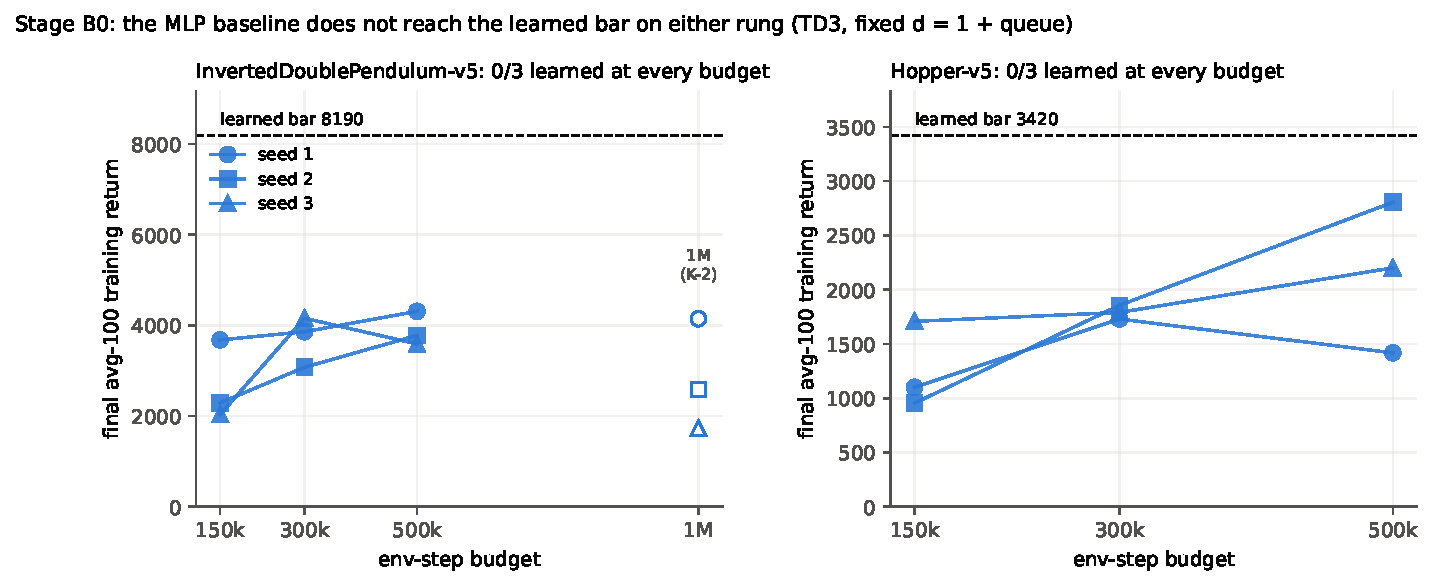
\includegraphics[width=\linewidth,height=0.42\textheight,keepaspectratio]{figures/p4_f2_b0_pilots.pdf}
\caption{Stage B0: final avg-100 by budget on IDP (with the 1M diagnostic) and on Hopper, against each rung's learned bar}
\end{figure}



\section*{3. The Hopper fallback (KB0)}



The author fired the kill switch on 2026-10-07, day 2 (amendment K-1), and the Hopper-v5 pilot ran as pre-registered: same budgets and seeds, MLP, TD3, C1, threshold unchanged at 3420.



\begin{center}\small\begin{tabular}{>{\raggedright\arraybackslash}p{0.069\linewidth}>{\raggedright\arraybackslash}p{0.275\linewidth}>{\raggedleft\arraybackslash}p{0.081\linewidth}>{\raggedright\arraybackslash}p{0.257\linewidth}>{\raggedright\arraybackslash}p{0.169\linewidth}}
\toprule
Budget & Final avg-100, seeds 1 / 2 / 3 & Learned & Eval last-5, seeds 1 / 2 / 3 & Wall-clock (min) \\
\midrule
150k & 1101.1 / 954.0 / 1708.2 & 0/3 & 1022.3 / 1102.5 / 2481.4 & 8.7 / 14.3 / 8.7 \\
300k & 1729.6 / 1855.6 / 1790.4 & 0/3 & 2961.6 / 2085.1 / 2031.1 & 19.4 / 30.3 / 19.4 \\
500k & 1418.0 / 2805.3 / 2201.3 & 0/3 & 2268.1 / 2649.8 / 3048.2 & 32.5 / 32.5 / 34.5 \\
\bottomrule
\end{tabular}\end{center}



\emph{Source: \texttt{experiments/\allowbreak{}analysis\_\allowbreak{}p4\_\allowbreak{}b0h.\allowbreak{}json}.}



\textbf{KB0: fail.} The best final is 2805.3 (seed 2, 500k), 82\% of the bar. The plan had flagged this risk in advance: Fujimoto et al. (2018) report about 3564 for TD3 on Hopper after 1M steps, so 3420 in noisy training return at $\leq$ 500k was likely out of reach. Hopper's untrained reference is 16.32 (R-2), so here too the MLP learns a great deal without reaching the bar. Per amendment K-2 the author dropped the Hopper rung.



\section*{4. The IDP diagnostic (B0d, amendment K-2)}



K-2 asked two questions of IDP before any decision on B1: does a much larger budget fix C1, and is the delay the obstacle? MLP, TD3, seeds 1--3; C1 at 1M steps, and no delay at 500k. Reported against the unchanged 8190 bar; no gate of its own.



\begin{center}\small\begin{tabular}{>{\raggedright\arraybackslash}p{0.078\linewidth}>{\raggedright\arraybackslash}p{0.167\linewidth}>{\raggedleft\arraybackslash}p{0.083\linewidth}>{\raggedright\arraybackslash}p{0.139\linewidth}>{\raggedright\arraybackslash}p{0.167\linewidth}>{\raggedright\arraybackslash}p{0.189\linewidth}}
\toprule
Arm & Final avg-100, seeds 1 / 2 / 3 & Learned (final) & Best avg-100 at any point & First step with avg-100 $\geq$ 8190 & Last 30 deterministic evals solved \\
\midrule
C1, 1M steps & 4146.9 / 2590.2 / 1732.8 & 0/3 & 5593.9 / 4940.4 / 5093.4 & never & 11 / 9 / 9 of 30 \\
No delay, 500k & 8226.2 / 5516.8 / 5779.7 & 1/3 & 9238.6 / 9144.9 / 9131.9 & 106,068 / 105,798 / 249,276 & 23 / 26 / 24 of 30 \\
\bottomrule
\end{tabular}\end{center}



\emph{Source: \texttt{experiments/\allowbreak{}analysis\_\allowbreak{}p4\_\allowbreak{}b0d.\allowbreak{}json}. A deterministic eval counts as solved at return > 9000.}



\begin{itemize}
\item \textbf{More budget does not fix C1.} At 1M steps no seed is learned, and 1M is no better than 300k--500k. After the first 100k steps, the per-100k-window share of full solves moves between 5.7\% and 48.5\% without a trend, and the avg-100 at the end of each window ranges from 1007.7 to 5130.6. The curves show repeated collapse and recovery rather than slow convergence.
\item \textbf{Without delay the same MLP reaches the bar.} All three seeds cross 8190 at some point (two by about 106k steps, the third by 249k), and best avg-100 exceeds 9100 in every seed. But the runs do not hold it: TD3 collapses and recovers here too (seed 1 falls from 8085.2 at 300k to 2907.5 at 400k, then returns to 8155.5), and only seed 1 ends above the bar.
\item \textbf{The one-step delay on an unstable plant is the main obstacle.} The deterministic policy solves about three in four evaluation episodes without delay (23--26 of 30) and about one in three with it (9--11 of 30). The delay costs most of the reliability, even with the pending action in the observation.
\end{itemize}



\begin{figure}[htbp]\centering
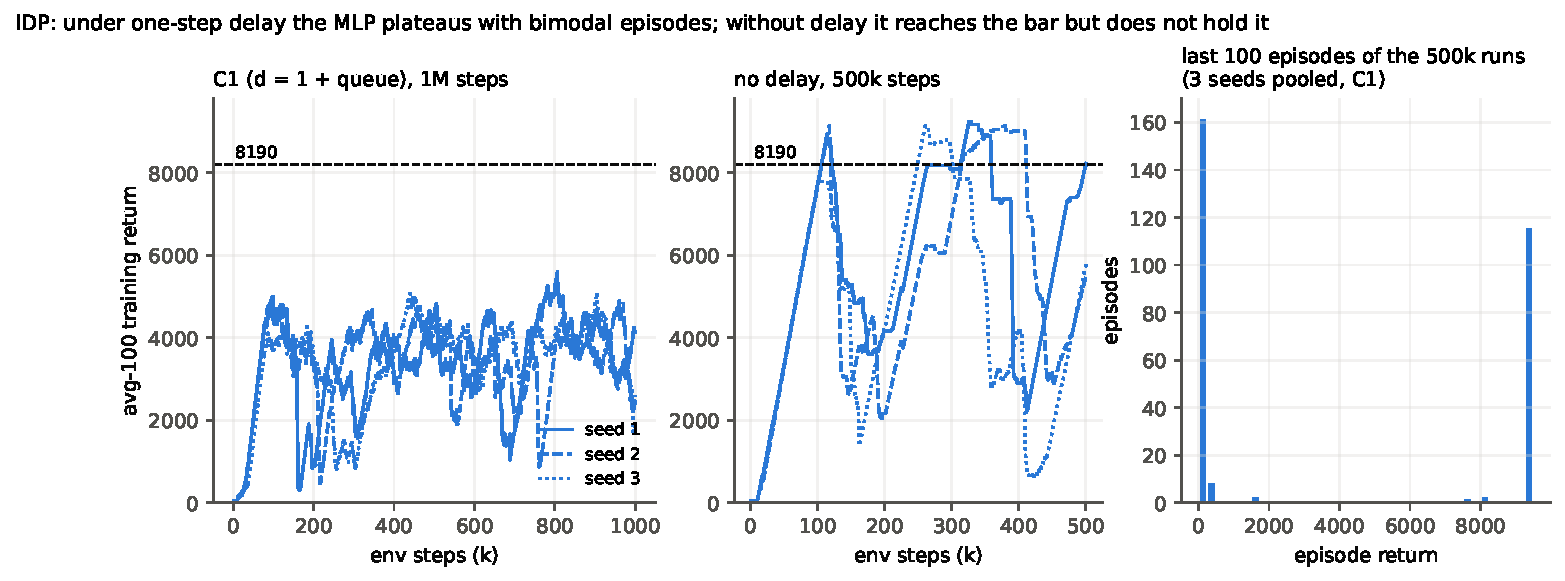
\includegraphics[width=\linewidth,height=0.42\textheight,keepaspectratio]{figures/p4_f3_idp_diagnostic.pdf}
\caption{IDP diagnostic: avg-100 under C1 for 1M steps and without delay for 500k, and the bimodal return distribution of the last 100 episodes at 500k}
\end{figure}



\section*{5. What happened next}



The 1M diagnostic did not pass GB0's rule (0/3), so under K-2 B1 could only have run as an exploratory study with a post-hoc "clear of floor" criterion. A draft amendment (\texttt{phase4/\allowbreak{}plan/\allowbreak{}K-3\_\allowbreak{}draft.\allowbreak{}md}) proposed that. The author decided on 2026-10-08 (amendment K-3) not to run B1 at all, for two reasons recorded in \texttt{gates.json}: no rung above Pendulum was learnable by the baseline under the pre-registered conditions, and Stage T had meanwhile shown that TRM 788k does not train under \texttt{td3.yaml} even on Pendulum, so a TD3 B1 on IDP would most likely have measured that optimisation failure rather than complexity scaling. The draft is superseded. \textbf{H1$'$ is recorded as not run, and H1 remains untested for the project.}



\section*{6. Threats to validity}



\begin{itemize}
\item \textbf{The bar is strict for noisy training return.} 8190 in avg-100 \emph{training} return includes TD3's exploration noise; deterministic evaluation is higher. The bar was fixed before data and is reported as fixed. The IDP diagnostic shows that the failure is not only an artefact of the metric: even greedy policies solve only a third of episodes under delay.
\item \textbf{One algorithm configuration.} TD3 ran with \texttt{td3.yaml} unchanged. A different learning rate, batch size or exploration scale might stabilise IDP. None was tried, by design.
\item \textbf{Three seeds.} Every B0 conclusion rests on n = 3 per budget. The failure is uniform (0/3 at every budget; none of the 21 C1 runs in B0, B0h and B0d learned), so the small n does not change the verdict.
\item \textbf{Hardware.} B0 runs landed on three GPU models, and results differ across models (\S{}2). Budgets were not run on a single model.
\end{itemize}



\section*{7. What B0 does and does not show}



It shows that, under the project's pre-registered conditions (TD3 as configured, one-step delay with the queue, $\leq$ 1M steps), neither IDP nor Hopper is learned reliably by the MLP baseline, and that on IDP the delay rather than the budget is the binding constraint. It does \textbf{not} show anything about TRM on these rungs: no TRM training run beyond the two 15k-step timing runs was made. In particular it is not evidence that TRM's relative deficit grows, shrinks or stays constant with complexity. That question, H1, is untested.



\subsection*{References}



Fujimoto, S., van Hoof, H. \& Meger, D. (2018). \emph{Addressing Function Approximation Error in Actor-Critic Methods.} ICML $\cdot$ Towers, M. et al. (2024). \emph{Gymnasium.} arXiv:2407.17032
\end{document}
